\documentclass[12pt]{beamer}
\usepackage[utf8]{inputenc}
\usepackage[T1]{fontenc}
\usepackage{lmodern}
\usepackage[spanish]{babel}
\usepackage{amsmath}
\usepackage{amsfonts}
\usepackage{amssymb}
\usepackage{graphicx}
\usepackage{hyperref}
\usetheme{Madrid}
\begin{document}
	\author{Fernando Oleo Blanco}
	\title{Introducción a Linux}
	%\subtitle{}
	%\logo{}
	\institute{ICAI - LinuxEC}
	\date{\today}
	%\subject{}
	%\setbeamercovered{transparent}
	\setbeamertemplate{navigation symbols}{}
\begin{frame}
	\maketitle
\end{frame}

\begin{frame}{Índice}
	\tableofcontents
\end{frame}

\section{Historia}

\subsection{UNIX}
\begin{frame}{UNIX}
	\begin{block}{Inicios}
		Nacido a finales de los años 60, principios de los 70. Creado por Bell Labs, y uno de los grupos más dotados de la historia de la computación. Es la semilla de los OSs modernos.
	\end{block}
	\begin{columns}
		\begin{column}{0.5\textwidth}
			\begin{figure}
				\centering
				\href{http://cat-v.org/}{\includegraphics[width=\linewidth]{Ken-Thompson-og-Dennis-Ritchie}}
				\caption{Ken Thompson \& Dennis Ritchie (Creador de C)}
				\label{fig:ken-thompson-og-dennis-ritchie}
			\end{figure}
		\end{column}
		\begin{column}{0.5\textwidth}
			\begin{figure}
				\centering
				\href{https://www.youtube.com/watch?v=QFK6RG47bww&list=PLzH6n4zXuckqZ90zLyy36qjO5YIn1RulG}{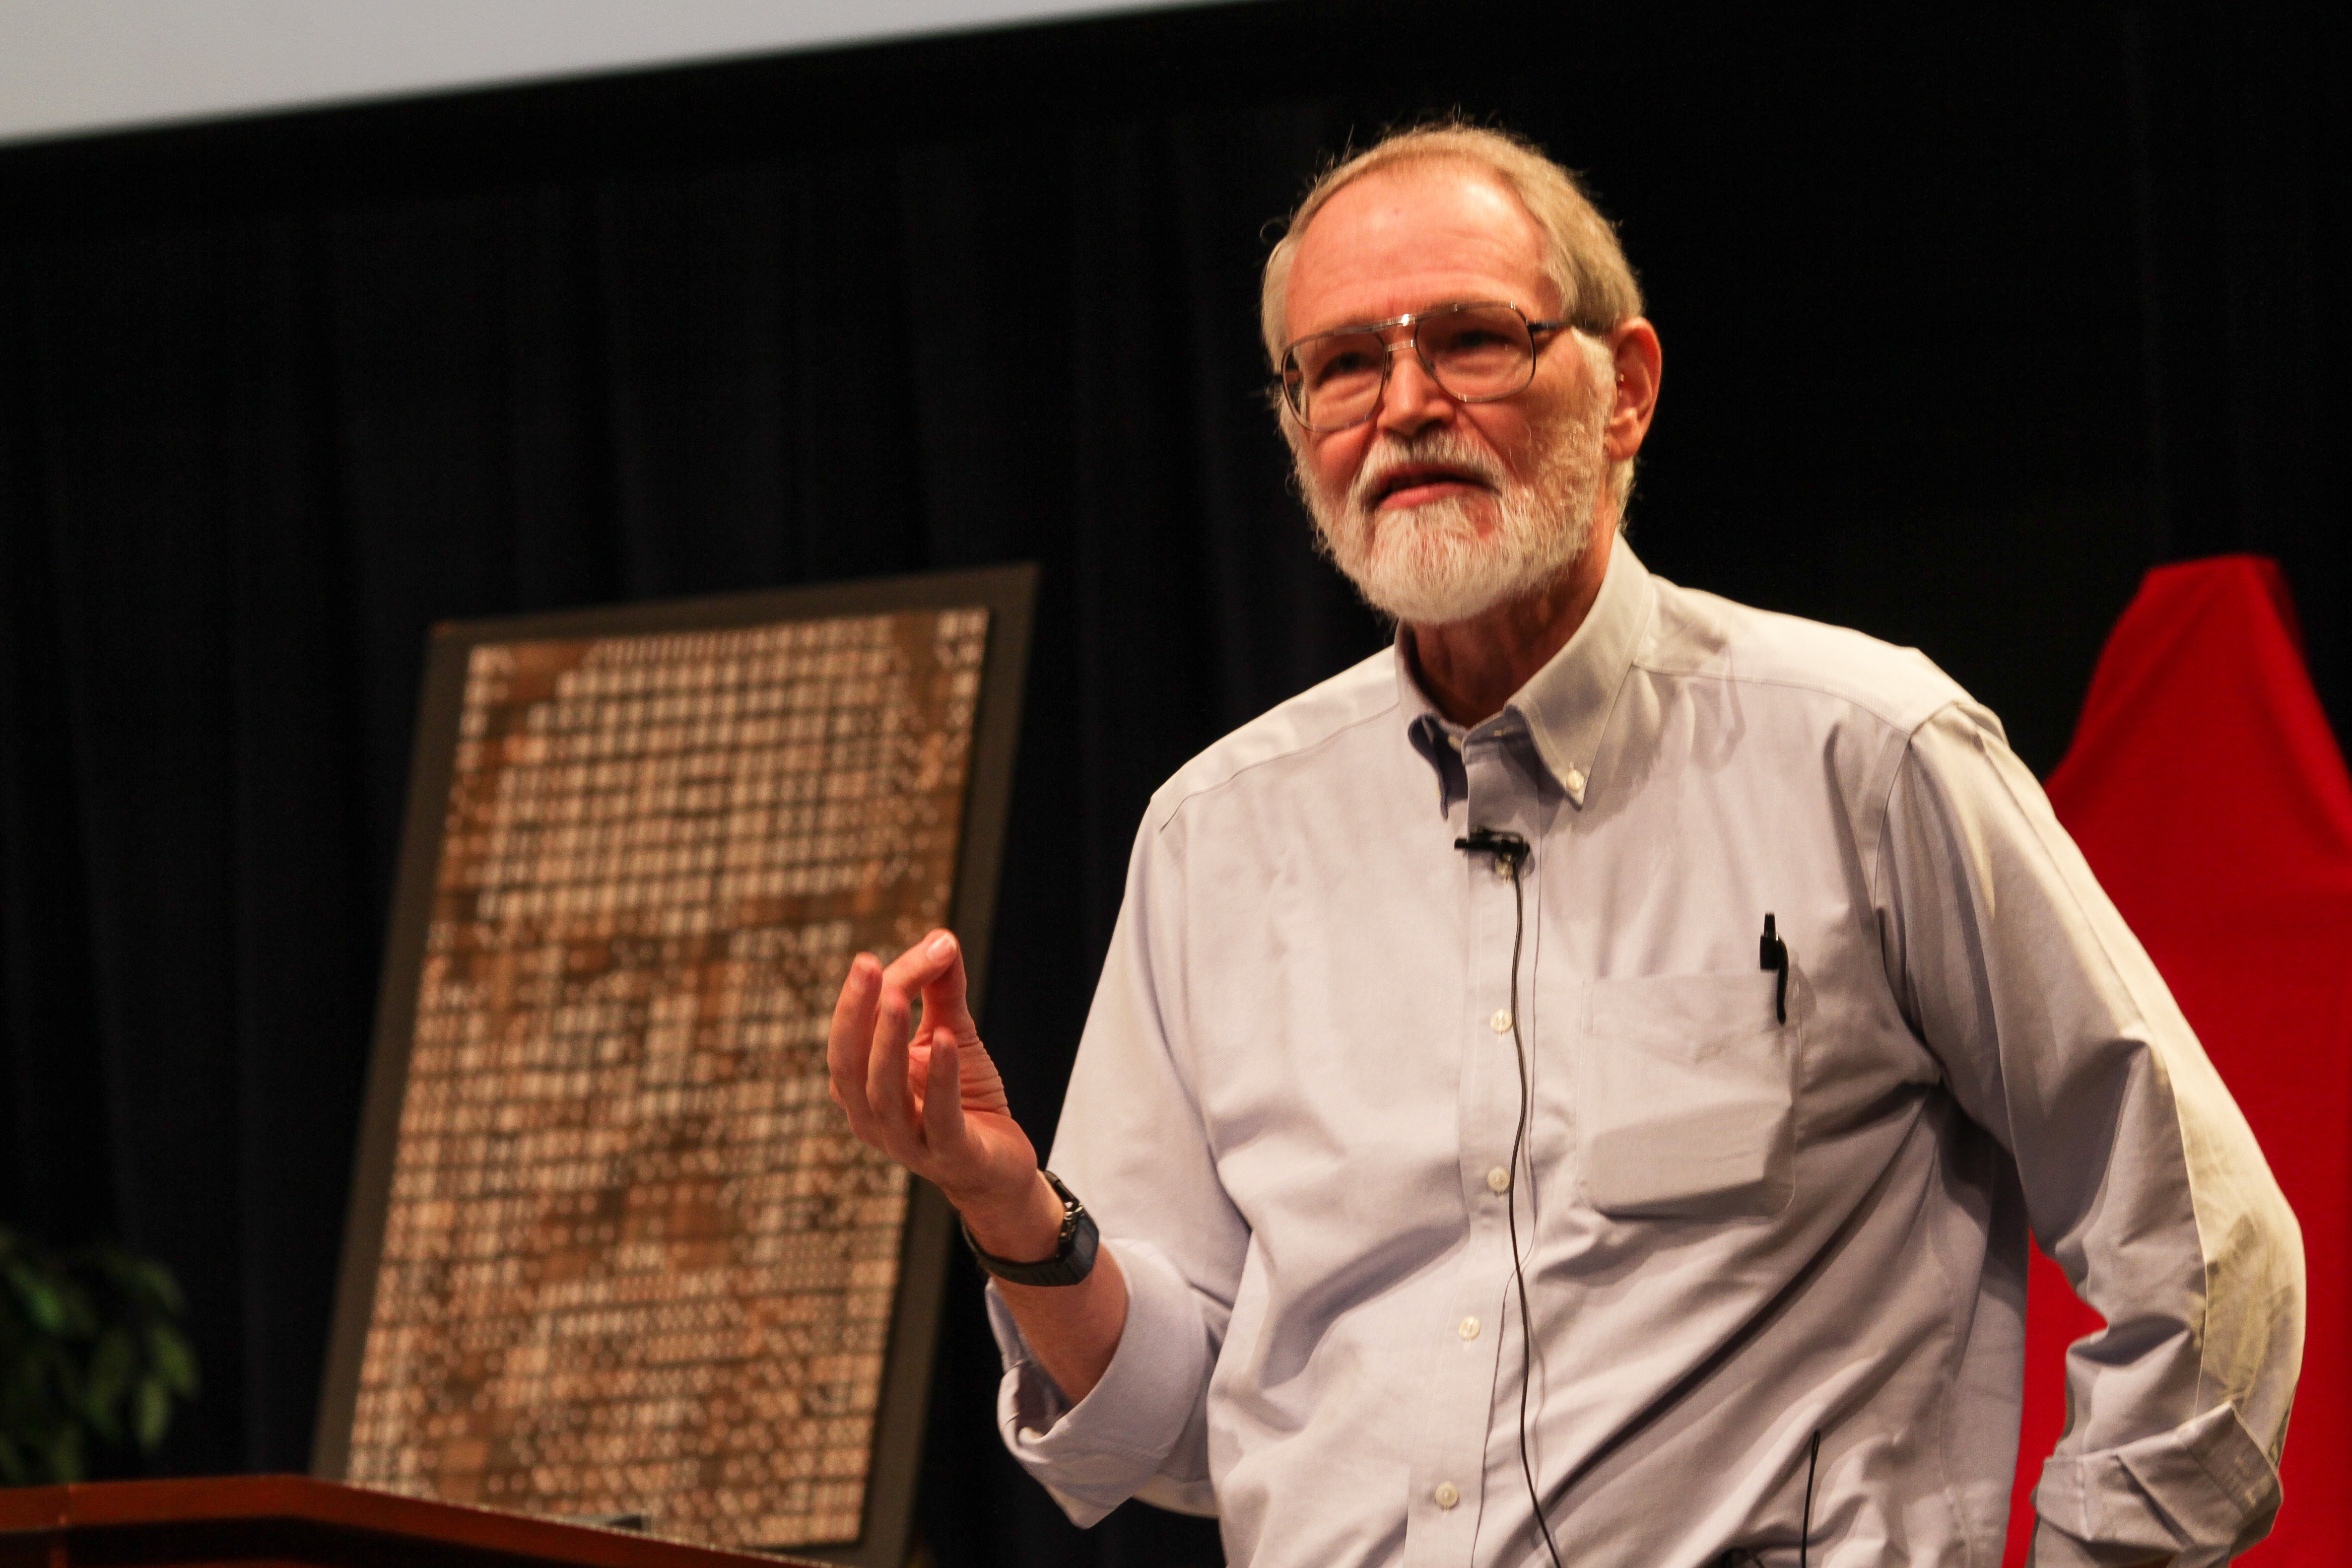
\includegraphics[width=\linewidth]{Brian_Kernighan_in_2012_at_Bell_Labs_1}}
				\caption{Brian Kernighan}
				\label{fig:briankernighanin2012atbelllabs1}
			\end{figure}
		\end{column}
	\end{columns}
	
\end{frame}

\subsection{GNU/FSF}
\begin{frame}{GNU}
	\begin{block}{GNU}
		Stallman, trabajando en el MIT anuncia ``\textit{the GNU Proyect}" en 1983, en el 84 empieza su desarrollo. El objetivo es tener un sistema completamente \textbf{libre}; ver \href{https://www.gnu.org/gnu/manifesto.html}{\textit{GNU's Manifesto}}. \textit{GNU is Not UNIX}. 
	\end{block}
	\begin{columns}
		\begin{column}{0.5\textwidth}
			\begin{figure}
				\centering
				\href{https://www.stallman.org/}{\includegraphics[width=\linewidth]{anopensourcelabel}}
				\caption{Richard Stallman}
				\label{fig:anopensourcelabel}
			\end{figure}
		\end{column}
		\begin{column}{0.5\textwidth}
			\begin{figure}
				\centering
				\href{https://www.youtube.com/watch?v=1jPmnDZ6ab8}{\includegraphics[width=0.7\linewidth]{FlICmGnj}}
				\caption{St. IGNcius}
				\label{fig:flicmgnj}
			\end{figure}
		
		\end{column}
	\end{columns}
\end{frame}

\begin{frame}{FSF}
	\begin{block}{Free Software Foundation}
		Fundación creada para la defensa del software \textbf{libre}. Da fondos a proyectos GNU, apoyo legal y hace campañas en contra de sus intereses y sirve como organismo \textit{regulador.}
	\end{block}
\begin{columns}
	\begin{column}{0.5\textwidth}
	\begin{figure}
		\centering
		\href{https://www.gnu.org/licenses/license-list.html}{\includegraphics[width=0.5\linewidth]{gerwinski-gnu-head}}
		\caption{Logo GNU}
		\label{fig:gerwinski-gnu-head}
	\end{figure}
\end{column}
\begin{column}{0.5\textwidth}
	\begin{figure}
		\centering
		\href{https://www.fsf.org/}{\includegraphics[width=0.7\linewidth]{fsf}}
		\caption{FSF}
		\label{fig:fsf}
	\end{figure}
	
\end{column}
\end{columns}

\end{frame}

\subsection{Linux}
\begin{frame}
	
\end{frame}

\section{Distribuciones/\textit{Distros}}
\begin{frame}
	content...
\end{frame}

\subsection{Desktop Environments}
\begin{frame}
	content...
\end{frame}

\section{Instalación}
\begin{frame}
	content...
\end{frame}

\section{Uso}
\begin{frame}
	content...
\end{frame}

\subsection{Continuará}
\begin{frame}
	content...
\end{frame}

\begin{frame}{Fin}
	content...
\end{frame}

\end{document}